\chapter{Cap\'{\i}tulo 2: Distribuci\'{o}n ZOIP} \label{cap2}
%{\Huge \textbf{Distribuci\'{o}n ZOIP\\}}

En modelaci\'{o}n estad\'{\i}stica es posible encontrarnos con variables respuesta como proporciones, porcentajes o tasas que se encuentran en el intevalo (0, 1). La distribuci\'{o}n m\'{a}s utilizada en la literatura para caracterizar este tipo de variables es la distribuci\'{o}n beta con soporte en el intervalo (0,1), la cual ha sido reparametrizada por autores como \cite{Ferrari2} y \cite{Stasinopoulos2}; otras distribuciones no tan comunes en la literatura pero que caracterizan este tipo de variables son la distribuci\'{o}n simplex \citep{Jorgensen1}, beta-rectangular \citep{Hahn1} y la distribuci\'{o}n LogitSep \citep{Hossain1}. Por otra parte, es com\'{u}n que los porcentajes o proporciones puedan dar valores iguales a cero o uno, re\-pre\-sen\-tan\-do la ausencia o presencia total de la caracter\'{\i}stica de inter\'{e}s, respectivamente, Las distribuciones descritas anteriormente no pueden ser admisibles para este tipos de variables, es por esto que se han desarrollado distribuciones infladas con ceros y/o unos, para tratar estos casos, como lo hizo \cite{Ospina2} quienes presentan una distribuci\'{o}n beta inflada en la que hacen una combinaci\'{o}n entre una distribuci\'{o}n discreta para la parte de los valores que pueden tomar cero o uno y una parte continua para los valores continuos entre cero y uno. \cite{Stasinopoulos2} incluyen dentro de sus modelos gamlss la distribuci\'{o}n beta inflada con ceros y/o unos seg\'{u}n su parametrizaci\'{o}n.\\

Esto ha dado pie para que diferentes autores hayan empezado a desarrollar diferentes mo\-de\-los de regresi\'{o}n para tratar este tipo variables, \cite{Ospina1} propusieran una clase general de modelos de regresi\'{o}n beta inflados con cero o uno, adem\'{a}s \cite{Kosmidis1} han estudiado dichos modelos inflados recientemente, pero con una distribuci\'{o}n distinta a la presentada por \cite{Ospina1}. \cite{Galvis1} presentan modelos de regresi\'{o}n para diferentes distribuciones para datos proporcionales inflados con ceros y/o unos mediante metodolog\'{\i}as de estimaci\'{o}n bayesianas.\\

Muchos autores han implementado distribuciones para datos proporcionales en el software estad\'{\i}stico \proglang{R}, \cite{Zeileis1} implementan el paquete \pkg{betareg} donde se encuentran los modelos de regresi\'{o}n beta propuestos por \cite{Ferrari2}, \cite{Qiu1} implementan el paquete \pkg{simplexreg} para realizar an\'{a}lisis de distribuci\'{o}n y regresi\'{o}n sobre una distribuci\'{o}n simplex, para datos proporcionales no inflados, otros autores como \citep{Stasinopoulos1} incluyen en el paquete \pkg{gamlss} la distribuci\'{o}n beta inflada con ceros y/o unos y la posibilidad de realizar modelos de regresi\'{o}n sobre ellos.\\

Aunque muchos autores han implementado las distribuciones para datos proporcionales inflados con ceros y/o unos, ninguno ha presentado una propuesta como la de reunir en una sola distribuci\'{o}n las diferentes distribuciones para datos proporcionales y sus diferentes parametrizaciones, adem\'{a}s de implementarla en un solo paquete, como se presenta en el paquete \pkg{ZOIP} en \cite{R} disponible en el repositorio web \verb|GitHub|.\\

El cap\'{\i}tulo se encuentra organizado de la siguiente manera: primero se presentan las distribuciones m\'{a}s representativas para datos proporcionales, en la siguiente secci\'{o}n se presenta la distribuci\'{o}n para datos proporcionales inflados con ceros y/o unos ZOIP (Zeros Ones Inflated Proportional), seguido por el desarrollo anal\'{\i}tico de la estimaci\'{o}n de los par\'{a}metros de la distribuci\'{o}n ZOIP v\'{\i}a m\'{a}xima verosimilitud, luego se presenta la forma de utilizar el paquete \pkg{ZOIP} para ajustar una distribuci\'{o}n ZOIP, por \'{u}ltimo se aplica el ajuste de una distribuci\'{o}n ZOIP en un estudio de simulaci\'{o}n y para datos reales.

%%%%%%%%%%%%%%%%%%%%%%%%%%%%%%%%%%%%%%%%%%%%%%%%%%%%%%%%%%%%%%%%%%%%%%%%%%%%%%%%%%%%%%%%%%%%%%%%%%%%%%%%%%%%%%%%%%%%%%%%%%%%%%%%%%%%%%%%%%%%%%%%%%%%%%%%%%%%%%%%%%

\section{Distribuci\'{o}n para datos proporcionales} \label{Sec_dist_prop}

Para los casos de modelaci\'{o}n donde la variable de inter\'{e}s es una proporci\'{o}n, un porcentaje o una tasa. Este tipo de variables no pueden ser analizadas con la distribuci\'{o}n normal, debido a que el soporte de la normal es la recta real $\mathbb{R}$, adem\'{a}s en este tipo de variables es com\'{u}n la asimetr\'{\i}a e incluso la bimodalidad, por esta raz\'{o}n en la literatura estad\'{\i}stica se han propuesto distribuciones para este tipo de comportamientos, como la distribuci\'{o}n beta, que cuenta con diferentes parametrizaciones (\cite{Ferrari2} y \cite{Stasinopoulos2}) y la distribuci\'{o}n simplex propuesta por \cite{Barndorff1}, de igual manera otras distribuciones m\'{a}s particulares como la beta-rectangular \citep{Hahn1} y LogitSep \citep{Hossain1} se acoplan a este comportamiento, a continuaci\'{o}n se mostraran las funciones de densidad de probabilidad, la media, la varianza y dependencias de algunas de las distribuciones mencionadas anteriormente.

\subsection{Distribuci\'{o}n beta original}

Si una variable aleatoria $y$ definida entre cero y uno, tiene distribuci\'{o}n beta con par\'{a}metros $p$ y $q$ se acostumbra a denotarla por $y \sim$ Be$(p,q)$ y la funci\'{o}n de densidad de probabilidad de la distribuci\'{o}n es dada por:
\begin{equation}
f(y;p,q)=\frac{\Gamma(p+q)}{\Gamma(p)\Gamma(q)}y^{p-1}(1-y)^{q-1}
\end{equation}

donde los par\'{a}metros $p>0$, $q>0$ y $\Gamma(\cdot)$ es la funci\'{o}n gamma. El valor esperado y la varianza de \textit{y} est\'{a}n dadas por:

\begin{align}
\begin{split}
	E(y) &= \frac{p}{p+q} 
\end{split} \label{E_Origin} \\
\begin{split}
	Var(y) &= \frac{pq}{(p+q)^2(p+q+1)}
\end{split} \label{V_Origin}
\end{align}


\subsection{Distribuci\'{o}n beta parametrizaci\'{o}n Ferrari y Cribari-Neto (2004)}


\cite{Ferrari2} propusieron otra parametrizaci\'{o}n para la distribuci\'{o}n beta en funci\'{o}n de los par\'{a}metos $\mu$ y $\phi$ donde $\mu$ corresponde a la media de la distribuci\'{o}n y $\phi$ es interpretado como un par\'{a}metro de precisi\'{o}n. Si $0<y<1$ y $Y \sim$ Be$(\mu,\phi)$ la funci\'{o}n de densidad de probabilidad de la distribuci\'{o}n est\'{a} dada por:
\begin{equation}
f(y;\mu,\phi)=\frac{\Gamma(\phi)}{\Gamma(\mu\phi)\Gamma((1-\mu)\phi)}y^{\mu\phi-1}(1-y)^{(1-\mu)\phi-1}
\end{equation}

donde $0<\mu<1$ y $\phi>0$. El valor esperado y la varianza de \textit{y} est\'{a}n dados por:

% Si $\mu=1/2$ la distribuci\'{o}n es sim\'{e}trica y si $\mu\neq1/2$ es asim\'{e}trica, adem\'{a}s cuando $\mu=1/2$ y $\phi=2$ se convierte en la distribuci\'{o}n uniforme y para valores m\'{a}s grandes de $\phi$ la varianza de $y$ es m\'{a}s peque\~{n}a

\begin{align}
\begin{split}
	E(y) &= \mu 
\end{split} \label{E_FC} \\
\begin{split}
	Var(y) &= \frac{\mu(1-\mu)}{1+\phi}
\end{split} \label{V_FC}
\end{align}

Adem\'{a}s note que la parametrizacion de la distribuci\'{o}n beta original es equivalente a la de \cite{Ferrari2} cuando:

\begin{align}
\begin{split}
	p &= \mu\phi
\end{split} \label{FC_Origin1} \\
\begin{split}
q &= (1-\mu)\phi
\end{split} \label{FC_Origin2}
\end{align}

\subsection{Distribuci\'{o}n beta parametrizaci\'{o}n Rigby y Stasinopoulos (2005)}\label{Sec:Dist_rigby}

\cite{Stasinopoulos2} propusieron una nueva parametrizaci\'{o}n para la distribuci\'{o}n beta con par\'{a}metros $\mu$ y $\sigma$ donde $\mu$ es la media de la distribuci\'{o}n y $\sigma$ es interpretado como un par\'{a}metro de dispersi\'{o}n, se dice que $Y \sim$ Be$(\mu,\sigma)$ con $0<y<1$, si la funci\'{o}n de densidad de probabilidad de la distribuci\'{o}n est\'{a} dada por:

\begin{equation}
f(y;\mu,\sigma)=B(\mu,\sigma)y^{\mu((1-\sigma^2)/\sigma^2)-1}(1-y)^{(1-\mu)((1-\sigma^2)/\sigma^2)-1}
\end{equation}

donde $B(\mu,\sigma)=\frac{\Gamma((1-\sigma^2)/\sigma^2)}{\Gamma(\mu((1-\sigma^2)/\sigma^2))\Gamma((1-\mu)((1-\sigma^2)/\sigma^2))},$\\

donde $0<\mu<1$ y $0<\sigma<1$. La media y la varianza de \textit{y} est\'{a}n dadas por:

\begin{align}
\begin{split}
	E(y) &= \mu 
\end{split} \label{E_RS} \\
\begin{split}
	Var(y) &= \sigma^2\mu(1-\mu)
\end{split} \label{V_RS}
\end{align}

Adem\'{a}s note que la parametrizacion de la distribucion beta original es equivalente a la de \cite{Stasinopoulos2} cuando:

\begin{align}
\begin{split}
	p &= \frac{\mu(1-\sigma^2)}{\sigma^2}
\end{split} \label{RS_Origin1} \\
\begin{split}
q &= \frac{(1-\mu)(1-\sigma^2)}{\sigma^2} 
\end{split} \label{RS_Origin2}
\end{align}

\subsection{Distribuci\'{o}n simplex}

La distribuci\'{o}n simplex fue introducida por \cite{Barndorff1} y es un caso particular de los modelos de dispersi\'{o}n propuestos por \cite{Jorgensen1}, dicha distribuci\'{o}n depende de los par\'{a}metros $\mu$ que es la media de la distribuci\'{o}n y $\sigma^2$ que es un par\'{a}metro de dispersi\'{o}n. Si $0<y<1$ y $Y \sim S^{-}(\mu, \sigma^2)$ la funci\'{o}n de densidad de probabilidad esta dada por:

\begin{equation}
f(y;\mu,\sigma^2)=\left\{2\pi\sigma^2[y(1-y)]^3\right\}^{-1/2}\exp\left\{-\frac{y(1-y)\mu^2(1-\mu)^2}{2\sigma^2(y-\mu)^2}\right\}
\end{equation}

donde $0<\mu<1$ y $\sigma>0$. Adem\'{a}s el valor esperado y la varianza est\'{a}n dadas por:

\begin{align}
\begin{split}
	E(y) &= \mu 
\end{split} \label{E_Simplex} \\
\begin{split}
	Var(y) &= \mu(1-\mu)-\frac{1}{\sqrt{2\sigma^2}}\exp\left\{\frac{1}{2\sigma^2\mu^2(1-\mu)^2}\right\}\Gamma\left\{\frac{1}{2},\frac{1}{2\sigma^2\mu^2(1-\mu)^2}\right\}
\end{split} \label{V_Simplex}
\end{align}

donde $\Gamma(a,b)$ est\'{a} dado por la funci\'{o}n$-\Gamma$ incompleta definido como $\Gamma(a,b)=\int_{b}^{\infty}{t^{a-1}b^tdt}$. ver m\'{a}s en \cite{Zhang1}.

%%%%%%%%%%%%%%%%%%%%%%%%%%%%%%%%%%%%%%%%%%%%%%%%%%%%%%%%%%%%%%%%%%%%%%%%%%%%%%%%%%%%%%%%%%%%%%%%%%%%%%%%%%%%%%%%%%%%%%%%%%%%%%%%%%%%%%%%%%%%%%%%%%%%%%%%%%%%%%%%%%
\section{Distribuci\'{o}n ZOIP (Zeros Ones Inflated Proporcional)}\label{Sec_dist_zoip}

En las distribuciones vistas en la secci\'{o}n \ref{Sec_dist_prop}, se evidenciaron ciertas distribuciones que se ajustan al comportamiento de datos proporcionales, porcentajes o tasas que est\'{a}n en el intervalo (0,1), sin embargo, es com\'{u}n que estos datos tomen valores en cero y/o uno que representar\'{\i}an la ausencia o presencia total de cierta caracter\'{\i}stica, por lo que no ser\'{\i}a posible ajustar los datos a las distribuciones vistas anteriormente y es por eso que en este trabajo se propone la distribuci\'{o}n ZOIP, como un conjunto de distribuciones para datos proporcionales inflados con ceros y/o unos.

La distribuci\'{o}n para datos proporcionales inflados con ceros y/o unos se compone de la mezcla de tres distribuciones, dos de ellas discretas, que son distribuciones degeneradas en cero y uno, y una tercera distribuci\'{o}n continua que adem\'{a}s es una funci\'{o}n de densidad de probabilidad para datos proporcionales, como las presentadas anteriormente, si la variable aleatoria $y$ tiene distribuci\'{o}n ZOIP con par\'{a}metros $\mu$, $\sigma$, $p_0$ y $p_1$, se denotar\'{a} como $Y \sim ZOIP(\mu,\sigma, p_0, p_1)$, la funci\'{o}n de densidad de probabilidad est\'{a} dado por:

\begin{equation}
g(y;\mu,\sigma, p_{0}, p_{1})=
\begin{cases}
p_{0} & \text{si}\ y=0,\\
p_{1} & \text{si}\ y=1,\\
(1-p_{0}-p_{1})f(y;\mu,\sigma) & \text{si}\ y \in (0,1)
\end{cases}
 \label{eq_Dist_ZOIP}
\end{equation}

donde $p_{0} \geq 0$ representa la probabilidad que $y=0$ y $p_{1} \geq 0$ representa la probabilidad de que $y=1$, adem\'{a}s $0\leq p_{0}+p_{1}\leq 1$ y $f(y;\mu,\sigma)$ representa alguna de las funciones de densidad de probabilidad para datos proporcionales, descritas en la secci\'{o}n anterior. La media y varianza de $y$, est\'{a}n dadas por

\begin{equation}
	E(y) = p_1+(1-p_0-p_1)E^*(y)
\end{equation}

\begin{equation}
%\begin{multline}
	Var(y) = p_1(1-p1)+(1-p_0-p_1)\left[Var^*(y)+(p_0+p_1)[E^*(y)]^2-2E^*(y)p_1\right]
%\end{multline}
\end{equation}

donde $E^*(y)$ es el valor esperado de una distribuci\'{o}n para datos proporcionales como las des\-cri\-tas en \eqref{E_Origin}, \eqref{E_FC}, \eqref{E_RS} y \eqref{E_Simplex}. Adem\'{a}s la $Var^*(y)$ es la varianza de una distribuci\'{o}n para datos proporcionales como se muestra en \eqref{V_Origin}, \eqref{V_FC}, \eqref{V_RS} y \eqref{V_Simplex}.\\

Si para la distribuci\'{o}n $ZOIP(\mu, \sigma, p_0, p_1)$ se elige la distribuci\'{o}n beta con parametrizaci\'{o}n \cite{Ferrari2} entonces el par\'{a}metro $\sigma$ tomar\'{a} el rol del par\'{a}metro $\phi$ de la distribuci\'{o}n, si la parametrizaci\'{o}n es beta original $\mu$ y $\sigma$ tomar\'{a}n el rol de $p$ y $q$ respectivamente. En las dem\'{a}s distribuciones y parametrizaciones $\mu$ y $\sigma$ tomaran los valores y dominios correspondientes a su distribuci\'{o}n.\\

La distribuci\'{o}n ZOIP se encuentra inflada con ceros y unos, es decir bilateralmente, pero existe la posibilidad que hayan casos de estudio en que se encuentren datos inflados con unos \'{u}nicamente, por lo que $p_0=0$ y por lo tanto se estar\'{a} llamando no una distribuci\'{o}n ZOIP, sino una distribuci\'{o}n OIP (Ones Inflated Proporcional) y si los datos se encuentran inflados con ceros \'{u}nicamente, es decir $p_1=0$ se tendr\'{a} una distribuci\'{o}n ZIP (Zeros Inflated Proporcional), Si los datos no se encuentran inflados, entonces $p_0=p_1=0$ y la distribuci\'{o}n ZOIP ser\'{a} una distribuci\'{o}n para datos proporcionales cl\'{a}sica.\\

En la Figura \ref{Dist_ZOIP} se muestran las densidades para varias de las distribuciones ZOIP-beta en sus diferentes parametrizaciones y ZOIP-simplex, es de aclarar que en las Figuras 1a. 1b. 1c. los valores de los par\'{a}metros son diferentes pero dan como resultado la misma distribuci\'{o}n gracias a las ecuaciones descritas en \eqref{FC_Origin1}, \eqref{FC_Origin2} para el caso \cite{Ferrari2} y \eqref{RS_Origin1}, \eqref{RS_Origin2} para el caso \cite{Stasinopoulos2}. Adem\'{a}s se puede observar en la Figura 1d. como la distribuci\'{o}n ZOIP-simplex hereda el comportamiento bimodal de la distribuci\'{o}n cl\'{a}sica simplex, con valores m\'{\i}nimo y m\'{a}ximo en cero y uno respectivamente. 

\begin{figure}
	\begin{center}
		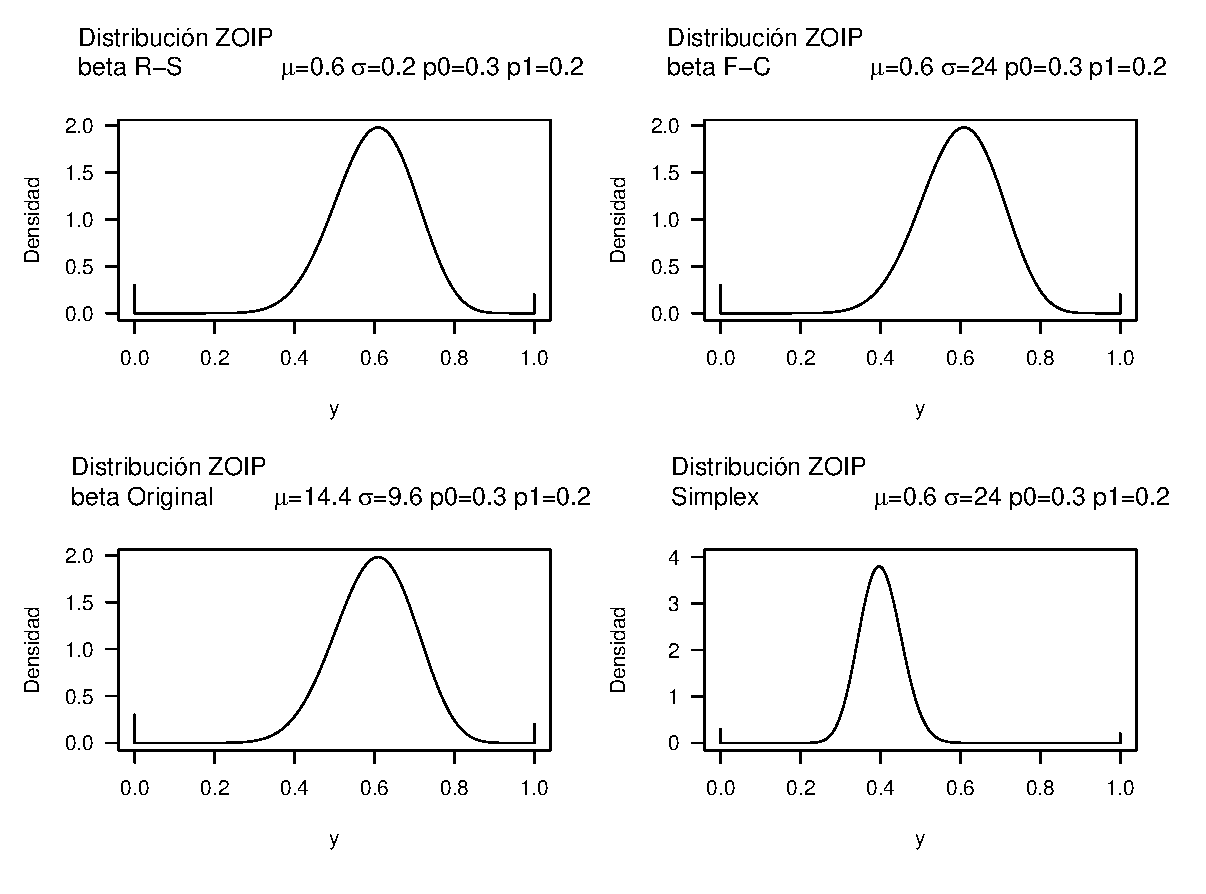
\includegraphics[scale=0.6]{Dist_ZOIP.eps}
		\caption{Densidades para la distribuci\'{o}n ZOIP para algunos valores de los par\'{a}metros, donde R-S se refiere a Rigby \& Stasinopoulos (2005) y F-C es Ferrari \& Cribari-Neto (2004).}
		\label{Dist_ZOIP}
	\end{center}
\end{figure}


%%%%%%%%%%%%%%%%%%%%%%%%%%%%%%%%%%%%%%%%%%%%%%%%%%%%%%%%%%%%%%%%%%%%%%%%%%%%%%%%%%%%%%%%%%%%%%%%%%%%%%%%%%%%%%%%%%%%%%%%%%%%%%%%%%%%%%%%%%%%%%%%%%%%%%%%%%%%%%%%%%
\section{Inferencia estad\'{\i}stica}

Para estimar los par\'{a}metros de la distribuci\'{o}n ZOIP se usa el m\'{e}todo de m\'{a}xima verosimilitud. La funci\'{o}n de verosimilitud para $\boldsymbol{\theta}=(\mu, \sigma, p_0, p_1)^{\top}$, basado en una muestra de $\boldsymbol{y}_i$ observaciones independientes, es de la forma:

\begin{equation}
L(\boldsymbol{\theta})=\prod_{i=1}^{n}g(\mathbf{y}_i;\mu, \sigma, p_0, p_1) 
\label{F_likel}
\end{equation}

%\[
%\ell(\boldsymbol{\theta})=\sum_{i=1}^{n}{\ell_i(\boldsymbol{\theta}) }
%\]

%donde para el caso de ZOIP-Beta original $\mu=p$, $\sigma=q$; si la distribuci\'{o}n ZOIP-Beta fuese con parametrizaci\'{o}n de \cite{Ferrari2} el \'{u}nico par\'{a}metro que cambiar\'{\i}a es $\sigma=\phi$, el resto de los par\'{a}metros no tendr\'{a}n modificaciones seg\'{u}n su parametrizaci\'{o}n o distribuci\'{o}n.\\

Para encontrar los estimadores de m\'{a}xima verosimilitud (MLE) de la distribuci\'{o}n ZOIP, se consideraran dos casos:

\begin{enumerate}
	\item \textbf{ZOIP-beta original}\\
	Considera la parametrizaci\'{o}n de la distribuci\'{o}n beta original y la ecuaci\'{o}n definida en \eqref{F_likel} se tiene que:
	\[
	\boldsymbol{\theta}=(p,q,p_0,p_1)^{\top}
	\]
	\[
	L(\boldsymbol{\theta})=\prod_{i=1}^{n}g(\boldsymbol{\theta}|y_i)=L_1(p_0)\cdot L_2(p_1) \cdot L_3(p,q)
	\]
	\\
Note que la funci\'{o}n de verosimilitud es factorizada en tres t\'{e}rminos, dos de ellos del componente discreto y uno compuesto por $p$ y $q$ del componente continuo, por tanto los par\'{a}metros son separables \citep{Pace1}, as\'{\i} la m\'{a}xima verosimilitud puede ser tratada por separado.\\
\[
L_1(p_0)=\prod_{i=1}^{n}p_0^{S_0(y_i)}(1-p_0)^{1-S_0(y_i)}=p_0^{\sum_{i=1}^{n}{S_0(y_i)}}(1-p_0)^{n-\sum_{i=1}^{n}{S_0(y_i)}}
\]
\\
donde:
\begin{equation}
S_j(y_i)=
\begin{cases}
1 & \text{si}\ y_i=j\\
0 & \text{si}\ y_i\neq j\\
\end{cases}
\quad ; \quad j=1,2 \label{Sj}
\end{equation}

Ahora sacando logaritmo natural a la funci\'{o}n de verosimilitud.
\[
\ell_1(p_0)=\sum_{i=1}^{n}{S_0(y_i)log(p_0)}+(n-\sum_{i=1}^{n}{S_0(y_i)})log(1-p_0)
\]	
\[
\frac{\delta \ell_1(p_0)}{\delta p_0}=\frac{\sum_{i=1}^{n}{S_0(y_i)}}{p_0}-\frac{n-\sum_{i=1}^{n}{S_0(y_i)}}{1-p_0}=\sum_{i=1}^{n}{S_0(y_i)}-p_0n=0
\]
\[
\hat{p}_0=\frac{1}{n}\sum_{i=1}^{n}{S_0(y_i)}
\]
\[
\therefore \hat{p}_1=\frac{1}{n}\sum_{i=1}^{n}{S_1(y_i)}
\]
\\
Ahora se halla MLE para los par\'{a}metros del componente continuo de la funci\'{o}n.

\[
\ell_3(p,q)=\sum_{i=1:y_i \in (0,1)}^{n}{log(f(p,q|y_i))}=n log(\Gamma(p+q))-n log(\Gamma(p))-n log(\Gamma(q))
\]
\[
+(p-1)\sum_{i=1:y_i \in (0,1)}^{n}{log(y_i)}+(q-1)\sum_{i=1:y_i \in (0,1)}^{n}{log(1-y_i)}
\]
\\
entonces
\[
\frac{\delta \ell_3(p,q)}{\delta p}=\sum_{i=1:y_i \in (0,1)}^{n}{log(y_i)}+\frac{n \cdot \delta log(\Gamma(p+q))}{\delta p}- \frac{n \cdot \delta log(\Gamma(p))}{\delta p}-\frac{n\cdot \delta log(\Gamma(q))}{\delta p}=0
\]
\[
\frac{\delta \ell_3(p,q)}{\delta q}=\sum_{i=1:y_i \in (0,1)}^{n}{log(1-y_i)}+\frac{n \cdot \delta log(\Gamma(p+q))}{\delta q}- \frac{n \cdot \delta log(\Gamma(p))}{\delta q}-\frac{n\cdot \delta log(\Gamma(q))}{\delta q}=0
\]

\[
\frac{\delta \ell_3(p,q)}{\delta p}=\sum_{i=1:y_i \in (0,1)}^{n}{log(y_i)}-n(-\psi(p+q)+\psi(p))=0
\]
\[
\frac{\delta \ell_3(p,q)}{\delta q}=\sum_{i=1:y_i \in (0,1)}^{n}{log(1-y_i)}-n(-\psi(p+q)+\psi(q))=0
\]
\\
donde $\psi(\cdot)={\Gamma^{'}{(\cdot)}}/{\Gamma(\cdot)}$
\\
Este sistema de ecuaciones no tiene una soluci\'{o}n de forma cerrada, por lo que para encontrar los MLE de $p$ y $q$ es necesario utilizar algoritmos iterativos, por ejemplo el m\'{e}todo de Newton Raphson, m\'{\i}nimos cuadrados ponderados y en el paquete \pkg{ZOIP} se utiliza optimizadores a la funci\'{o}n de verosimilitud mediante la funci\'{o}n \code{nlminb} de \proglang{R}, sin embargo, se puede garantizar que los puntos cr\'{\i}ticos encontrados ser\'{a}n m\'{a}ximos de la funci\'{o}n de verosimilitud, ya que si hallamos la segunda derivada de la funci\'{o}n se tiene que:
\[
\frac{\delta^2 \ell_3(p,q)}{\delta p^2}=-n(\psi^{'}(p)-\psi^{'}(p+q))<0
\]
\[
\frac{\delta^2 \ell_3(p,q)}{\delta q^2}=-n(\psi^{'}(q)-\psi^{'}(p+q))<0
\]
\\
debido que la varianza de la transformaci\'{o}n logar\'{\i}tmica de la variable es:
\[
var(log(y))=E[log^2(y)]-(E[log(y)])^2=\psi^{'}(p)-\psi^{'}(p+q)>0
\]
\[
var(log(1-y))=E[log^2(1-y)]-(E[log(1-y)])^2=\psi^{'}(q)-\psi^{'}(p+q)>0
\]
\\
ver m\'{a}s en \cite{Owen1}.\\

Para encontrar las estimaciones de los par\'{a}metros de beta en parametrizaciones de \cite{Ferrari2} y \cite{Stasinopoulos2}, basta con encontrar los estimadores MLE anteriores de la parametrizaci\'{o}n original y utilizar las ecuaciones definidas en \eqref{FC_Origin1}, \eqref{FC_Origin2} para el caso de \cite{Ferrari2} y \eqref{RS_Origin1}, \eqref{RS_Origin2} para el caso de \cite{Stasinopoulos2}.

\item \textbf{ZOIP-simplex}\\

Para este caso lo \'{u}nico que var\'{\i}a con respecto al anterior es la estimaci\'{o}n en el componente continuo.

\[
L_3(\mu,\sigma)=\prod_{i=1:y_i \in (0,1)}^{n}\left[{2\pi \sigma^{2}[y_i(1-y_i)]^{3}}\right]^{-1/2}exp\left(-\frac{1}{2\sigma^2}d(y_i;\mu)\right)
\]
\\
donde $d(y_i ;\mu)=\frac{y_i(1-y_i)\mu^2(1-\mu)^2}{(y_i-\mu)^2}$
\[
\ell_3(\mu,\sigma)=-\frac{n}{2}log(2\pi)-\frac{n}{2}log(\sigma^2)-\frac{3}{2}\sum_{i=1:y_i \in (0,1)}^{n}{log(y_i(1-y_i))}-\sum_{i=1:y_i \in (0,1)}^{n}{\frac{1}{2\sigma^2}d(y_i;\mu)}
\]

\[
\frac{\delta \ell_3(\mu,\sigma)}{\delta \sigma}=-\frac{n}{\sigma}+\frac{1}{\sigma^3}\sum_{i=1:y_i \in (0,1)}^{n}{d(y_i;\mu)}=\sigma(-n\sigma^2+\sum_{i=1:y_i \in (0,1)}^{n}{d(y_i;\mu))}=0
\]
\\
no es admisible que $\sigma=0$ entonces:
\[
-n\sigma^2+\sum_{i=1:y_i \in (0,1)}^{n}{d(y_i;\mu)}=0
\]
\[
\therefore \hat{\sigma}^2=\frac{1}{n}\sum_{i=1:y_i \in (0,1)}^{n}{d(y_i;\mu)}
\]
\\
El estimador MLE de $\sigma^2$ depende del valor estimado en $\mu$, entonces:
\[
\frac{\delta \ell_3(\mu,\sigma)}{\delta \sigma}=-\frac{1}{2\sigma^2}\sum_{i=1:y_i \in (0,1)}^{n}{\frac{\delta d(y_i;\mu)}{\delta\mu}}=0
\]

\begin{multline*}
\frac{\delta d(y_i;\mu)}{\delta\mu}=\sum_{i=1:y_i \in (0,1)}^{n}\frac{y_i(1-y_i)\mu^2(1-\mu)^2}{2(y_i-\mu)^3}\\
+\frac{2y_i(1-y_i)\mu(1-\mu)^2-2y_i(1-y_i)\mu^2(1-\mu)}{(y_i-\mu)^2}=0
\end{multline*}

No tiene una soluci\'{o}n cerrada anal\'{\i}ticamente, entonces se deben utilizar algoritmos iterativos tal como Newton Raphson o m\'{\i}nimos cuadrados ponderados, en el paquete \pkg{ZOIP} se utiliza optimizadores para la funci\'{o}n de verosimilitud mediante la funci\'{o}n \code{nlminb} de \proglang{R}, para encontrar puntos cr\'{\i}ticos donde ${\delta d(y_i;\mu)}/{\delta\mu}=0$.

\end{enumerate}

%%%%%%%%%%%%%%%%%%%%%%%%%%%%%%%%%%%%%%%%%%%%%%%%%%%%%%%%%%%%%%%%%%%%%%%%%%%%%%%%%%%%%%%%%%%%%%%%%%%%%%%%%%%%%%%%%%%%%%%%%%%%%%%%%%%%%%%%%%%%%%%%%%%%%%%%%%%%%%%%%%


\section{Distribuci\'{o}n ZOIP en el paquete \pkg{ZOIP}}

En esta secci\'{o}n se presenta el paquete \pkg{ZOIP} de \proglang{R} alojado en \verb|GitHub| y creado por los autores para analizar datos proporcionales inflados con ceros y/o unos y ajustar una distribuci\'{o}n ZOIP.

\subsection{Instalaci\'{o}n}

Para acceder a la \'{u}ltima versi\'{o}n del paquete \pkg{ZOIP}, se encuentra ubicada en \verb|GitHub|, el cual es un alojamiento de repositorios Git, para obtener dicha versi\'{o}n es necesario ejecutar el siguiente c\'{o}digo que instala el paquete \pkg{devtools}, que es necesario para descargar el paquete \pkg{ZOIP} y otros paquetes complementarios, para el correcto funcionamiento del paquete.

\begin{verbatim}
if (!require("devtools")) install.packages("devtools")
if (!require("rmutil")) install.packages("rmutil")
if (!require("boot")) install.packages("boot")
if (!require("numDeriv")) install.packages("numDeriv")
if (!require("GHQp")) install.packages("GHQp")
devtools::install_github("jucdiaz/ZOIP", force = TRUE)
library(ZOIP) # Carga el paquete
\end{verbatim}

\subsection{Funciones sobre distribuci\'{o}n ZOIP}

En el paquete \pkg{ZOIP} existen cuatro funciones llamadas \code{dZOIP}, \code{pZOIP}, \code{qZOIP} y \code{rZOIP} el cual corresponden a las funciones de densidad de probabilidad, la funci\'{o}n de distribuci\'{o}n acumulada, la funci\'{o}n cuantil y la funci\'{o}n generadora de n\'{u}meros aleatorios de la distribuci\'{o}n ZOIP, respectivamente; en el siguiente c\'{o}digo se observa como se halla la densidad de probabilidad en el punto $0.5$ de una distribuci\'{o}n ZOIP-beta con parametrizaci\'{o}n \cite{Stasinopoulos2} descrita como $\text{ZOIP}(\mu=0.2, \, \sigma=0.5, \, p_0=0.2, \, p_1=0.2)$\\

\begin{verbatim}
dZOIP(x = 0.5, mu = 0.2, sigma = 0.5, p0 = 0.2, p1 = 0.2, family = "R-S")
## [1] 0.3243543
\end{verbatim}

Adem\'{a}s se halla la probabilidad acumulada hasta el punto $0.5$ de una distribuci\'{o}n OIP-beta con parametrizaci\'{o}n \cite{Ferrari2} dada por $ZOIP(\mu=0.2, \, \sigma=3, \, p_0=0, \, p_1=0.2)$\\

\begin{verbatim}
pZOIP(q = 0.5, mu = 0.2, sigma = 3, p0 = 0, p1 = 0.2, family = "F-C")
## [1] 0.7181223
\end{verbatim}

Se calcula el percentil en el punto $0.7$ de una distribuci\'{o}n ZIP-beta original dada por $ZOIP(\mu=0.6, \, \sigma=2.4, \, p_0=0.2, \, p_1=0)$\\

\begin{verbatim}
qZOIP(p = 0.7, mu = 0.6, sigma = 2.4, p0 = 0.2, p1 = 0, 
    family = "Original")
## [1] 0.2061418
\end{verbatim}

Por \'{u}ltimo se generaron 8 valores aleatorios de una distribuci\'{o}n ZOIP-simplex descrita como $ZOIP(\mu=0.6, \, \sigma=3, \, p_0=0.2, \, p_1=0.2)$. La funci\'{o}n \code{set.seed} sirve para garantizar la repetici\'{o}n de los valores aleatorios generados en el ejemplo.\\

\begin{verbatim}
set.seed(12345)
rZOIP(n = 8, mu = 0.2, sigma = 3, p0 = 0.2, p1 = 0.2, family = "Simplex")
## [1] 0.3185479 1.0000000 0.3765073 1.0000000 0.1626598
## [6] 0.0000000 0.1138673 0.1840670
\end{verbatim}

\subsection{Funci\'{o}n RM.ZOIP}

La funci\'{o}n \code{RM.ZOIP} estima los par\'{a}metros de una distribuci\'{o}n ZOIP, v\'{\i}a m\'{a}xima verosimilitud utilizando el optimizador deseado (\code{nlminb}, \code{optim}). La estructura de la funci\'{o}n \code{RM.ZOIP} es la siguiente:

\begin{verbatim}
RM.ZOIP(formula.mu, formula.sigma = ~1, formula.p0 = ~1, 
    formula.p1 = ~1, data, link = c("identity", "identity", 
        "identity", "identity"), family = "R-S", optimizer = "nlminb")
\end{verbatim}

Los argumentos de la funci\'{o}n \code{RM.ZOIP} son:

\begin{itemize}[noitemsep, nolistsep]

\item \code{formula.mu}: Formula que define la funci\'{o}n de regresi\'{o}n para el par\'{a}metro $\mu$, Para ajustar una distibuci\'{o}n ZOIP debe tomar el valor de \code{y $\sim$ 1}, donde y es la variable a ajustar.
\item \code{formula.sigma}: Formula que define la funci\'{o}n de regresi\'{o}n para el par\'{a}metro $\sigma$, Para ajustar una distibuci\'{o}n ZOIP debe tomar el valor de \code{$\sim$ 1}.
\item \code{formula.p0}: Formula que define la funci\'{o}n de regresi\'{o}n para el par\'{a}metro $p_0$, Para ajustar una distibuci\'{o}n ZOIP debe tomar el valor de \code{$\sim $1}.
\item \code{formula.p1}: Formula que define la funci\'{o}n de regresi\'{o}n para el par\'{a}metro $p_1$,Para ajustar una distibuci\'{o}n ZOIP debe tomar el valor de \code{$\sim $1}.
\item \code{data}: Es el conjunto de datos en formato \code{data.frame} donde debe contener los datos de la variable a ajustar y el nombre debe ser la tal cual como est\'{a} en las f\'{o}rmula para el par\'{a}metro $\mu$.
\item \code{family}: Elecci\'{o}n de la distribuci\'{o}n ZOIP deseada para ajustar, si toma el valor de \code{``R-S''} se utilizar\'{a} la distribuci\'{o}n ZOIP-beta con parametrizaci\'{o}n  \cite{Stasinopoulos2}, si toma el valor de \code{``F-C''} se utilizar\'{a} la distribuci\'{o}n ZOIP-beta parametrizaci\'{o}n \cite{Ferrari2}, el valor de \code{``Original''} se utilizar\'{a} la distribuci\'{o}n ZOIP-beta con parametrizaci\'{o}n original, \code{``Simplex''} utilizar\'{a} la distribuci\'{o}n ZOIP-simplex.
\item \code{link}: Es un vector con las funciones enlace adecuadas para cada par\'{a}metro a estimar de acuerdo a las opciones escogidas en los par\'{a}metros de familia y formula. Para ajustar una distribuci i\'{o}n ZOIP se debe utilizar como funci\'{o}n enlace la opci\'{o}n \code{identity} en sus cuatro par\'{a}metros, independientemente de la distribuci i\'{o}n ZOIP escogida, en familia, por defecto \code{link=c(``identity'',``identity'',``identity'',``identity'')}.
\item \code{optimizer}: Elecci\'{o}n del optimizador, utilizado para encontrar la convergencia de la m\'{a}xima verosimilitud. se puede elegir el valor de \code{``nlminb''} o \code{``optim''}, por defecto \code{``nlminb''}
\end{itemize}

En el siguiente ejemplo se mostrara el ajuste de una distribuci\'{o}n ZOIP, para ello mostraremos la salida de la funci\'{o}n \code{RM.ZOIP} de $1000$ observaciones simuladas para la distribuci\'{o}n ZOIP-beta parametrizaci\'{o}n \cite{Stasinopoulos2}.\\

\begin{verbatim}
yi <- data.frame(yi = rZOIP(n = 1000, mu = 0.6, sigma = 0.2, 
    p0 = 0.03, p1 = 0.05, family = "R-S"))

mod <- RM.ZOIP(formula.mu = yi ~ 1, formula.sigma = ~1, 
    formula.p0 = ~1, formula.p1 = ~1, data = yi, family = "R-S")
mod
\end{verbatim}

\begin{verbatim}
## Call:
## RM.ZOIP(formula.mu = yi ~ 1, formula.sigma = ~1, formula.p0 = ~1, 
##     formula.p1 = ~1, data = yi, family = "R-S")
## 
##  Results: 
## 
##  Estimated coefficients for h(mu): 
## (Intercept) 
##    0.605174 
## 
##  Estimated coefficients for h(sigma): 
## (Intercept) 
##   0.2038938 
## 
##  Estimated coefficients for h(p0): 
## (Intercept) 
##  0.03000002 
## 
##  Estimated coefficients for h(p1): 
## (Intercept) 
##        0.05 
\end{verbatim}
\begin{verbatim}
## 
##  Convergence 
## [1] 0
## 
##  message 
## [1] "relative convergence (4)"
## 
##  iterations 
## [1] 22
## 
##  Log-likelihood 
## [1] 488.2683
\end{verbatim}

En el anterior resultado se obtienen varios aspectos importantes de la salida del ajuste de la distribuci\'{o}n y leyendo de arriba hacia abajo, primero que todo nos muestra la distribuci\'{o}n ajustada, luego para cada el valor ajustado para cada par\'{a}metro de la distribuci\'{o}n ZOIP, luego un indicador de convergencia del ajuste, donde 0 indica la convergencia, despu\'{e}s un mensaje sobre la convergencia (resultados heredados de la funci\'{o}n \code{nlimnb}), despu\'{e}s se encuentra el n\'{u}mero de iteraciones que fueron necesarias para que convergiera el ajuste de la distribuci\'{o}n, por \'{u}ltimo se encuentra valor de la log-verosimilitud que nos permitir\'{a} hacer comparaciones entre ajustes de distribuciones.\\ 

 Al aplicar a la distribuci\'{o}n ajustada (\code{mod}) la funci\'{o}n \code{summary} se obtiene el siguiente resultado:

\begin{verbatim}
summary(mod)
## ---------------------------------------------------------------
## Fixed effects for identity(mu)
## ---------------------------------------------------------------
##              Estimate Std. Error z value  Pr(>|z|)    
## (intercept) 0.6066914  0.0031636  191.78 < 2.2e-16 ***
## ---
## Signif. codes:  0 *** 0.001 ** 0.01 * 0.05 . 0.1   1
\end{verbatim}
\begin{verbatim}
## ---------------------------------------------------------------
## Fixed effects for identity(sigma)
## ---------------------------------------------------------------
##             Estimate Std. Error z value  Pr(>|z|)    
## (intercept) 0.196643   0.004322  45.498 < 2.2e-16 ***
## ---
## Signif. codes:  0 *** 0.001 ** 0.01 * 0.05 . 0.1   1
## ---------------------------------------------------------------
## Fixed effects for identity(p0)
## ---------------------------------------------------------------
##              Estimate Std. Error z value Pr(>|z|)    
## (intercept) 0.0339992  0.0057308  5.9327 2.98e-09 ***
## ---
## Signif. codes:  0 *** 0.001 ** 0.01 * 0.05 . 0.1   1
## ---------------------------------------------------------------
## Fixed effects for identity(p1)
## ---------------------------------------------------------------
##              Estimate Std. Error z value  Pr(>|z|)    
## (intercept) 0.0450005  0.0065556  6.8644 6.675e-12 ***
## ---
## Signif. codes:  0 *** 0.001 ** 0.01 * 0.05 . 0.1   1
## ---------------------------------------------------------------
## ---------------------------------------------------------------
\end{verbatim}
Con la funci\'{o}n \code{summary} aplicada a la distribuci\'{o}n ZOIP ajustada, se obtiene m\'{a}s detalles de los par\'{a}metros estimados, primero se obtiene el valor estimado (Estimate), su error est\'{a}ndar (Std.Error), el valor Z del estimador (z value) y el valor p que nos indicara la significancia del par\'{a}metro estimado (\code{Pr(>|z|)}).\\

En el resultado anterior se obtienen los valores de $\hat{\mu}=0.6066914$, $\hat{\sigma}=0.196643$, $\hat{p}_0=0.0339992$ y $\hat{p}_1=0.0450005$, que son a los par\'{a}metros con los que se simulo $y_i$. Adem\'{a}s cabe resaltar que en la funci\'{o}n \code{RM.ZOIP} para ajustar distribuciones de probabilidad no es necesario colocar funciones de enlace ni espacio de busqueda de los par\'{a}metros, ya que estos son introducidas autom\'{a}ticamente de acuerdo a el valor tomado en \code{family}.\\

As\'{\i} como la funci\'{o}n \code{summary} puede ser aplicada a un objeto de la clase \code{ZOIP} o \code{ZOIPM}, en este trabajo se implementaron otros tipo de funciones asociadas a m\'{e}todos S3 de \proglang{R} a objetos de clase \code{ZOIP} o clase \code{ZOIPM}, tales como la funci\'{o}n \code{print} y \code{coef}, que permiten mostrar los resultados del modelo ajustado en general y los par\'{a}metros regresores estimados, respetivamente.

%%%%%%%%%%%%%%%%%%%%%%%%%%%%%%%%%%%%%%%%%%%%%%%%%%%%%%%%%%%%%%%%%%%%%%%%%%%%%%%%%%%%%%%%%%%%%%%%%%%%%%%%%%%%%%%%%%%%%%%%%%%%%%%%%%%%%%%%%%%%%%%%%%%%%%%%%%%%%%%%%%

\section{Aplicaci\'{o}n}
En esta secci\'{o}n se muestran varios resultados sobre el ajuste de una distribuci\'{o}n ZOIP, primero se realiz\'{o} un estudio de simulaci\'{o}n para observar la convergencia de la estimaci\'{o}n de los par\'{a}metros de la distribuci\'{o}n, y en segunda instancia se ajust\'{o} una distribuci\'{o}n ZOIP a datos reales sobre la utilizaci\'{o}n de una tarjeta de cr\'{e}dito de una entidad financiera.

\subsection{Datos simulados}
En este estudio de simulaci\'{o}n se analizan diferentes aspectos de la capacidad de estimaci\'{o}n que tiene el m\'{e}todo de m\'{a}xima verosimilitud sobre los par\'{a}metros de la distribuci\'{o}n ZOIP. Se generaron muestras de una distribuci\'{o}n ZOIP bajo las diferentes distribuciones y par\'{a}metrizaciones con tama\~{n}os de muestra n de: 5, 10, 15 y as\'{\i} sucesivamente hasta 500, y se realizaron 1000 r\'{e}plicas para cada tama\~{n}o de muestra, posteriormente se calcul\'{o} la mediana de cada una de las estimaciones de los par\'{a}metros, y as\'{\i} poder analizar la capacidad de convergencia de las metodolog\'{\i}as implementadas en la distribuci\'{o}n ZOIP y en el paquete \pkg{ZOIP}.\\

En el primer escenario del estudio de simulaci\'{o}n se generaron los datos de una distribuci\'{o}n ZOIP-beta$(\mu=0.6 ,\sigma=0.2 , p_0=0.03 , p_1= 0.05)$ para el caso de la parametrizaci\'{o}n de \cite{Stasinopoulos2}, ZOIP-beta$(\mu=0.6 , \sigma=24 , p_0=0.03 , p_1= 0.05)$ para el caso de la parametrizaci\'{o}n de \cite{Ferrari2}, ZOIP-beta$(\mu=14.4 , \sigma=9.6 , p_0=0.03 , p_1= 0.05)$ en la parametrizaci\'{o}n original, cabe aclarar que las tres parametrizaciones anteriores generan exactamente la misma distribuci\'{o}n, esto gracias a las ecuaciones definidas en \eqref{FC_Origin1}, \eqref{FC_Origin2}, \eqref{RS_Origin1} y \eqref{RS_Origin2}, de igual manera se gener\'{o} la misma cantidad de datos simulados para la distribuci\'{o}n ZOIP-simplex$(\mu=0.4 , \sigma=0.2 , p_0=0.03 , p_1= 0.05)$.\\


\begin{figure}
	\begin{center}
		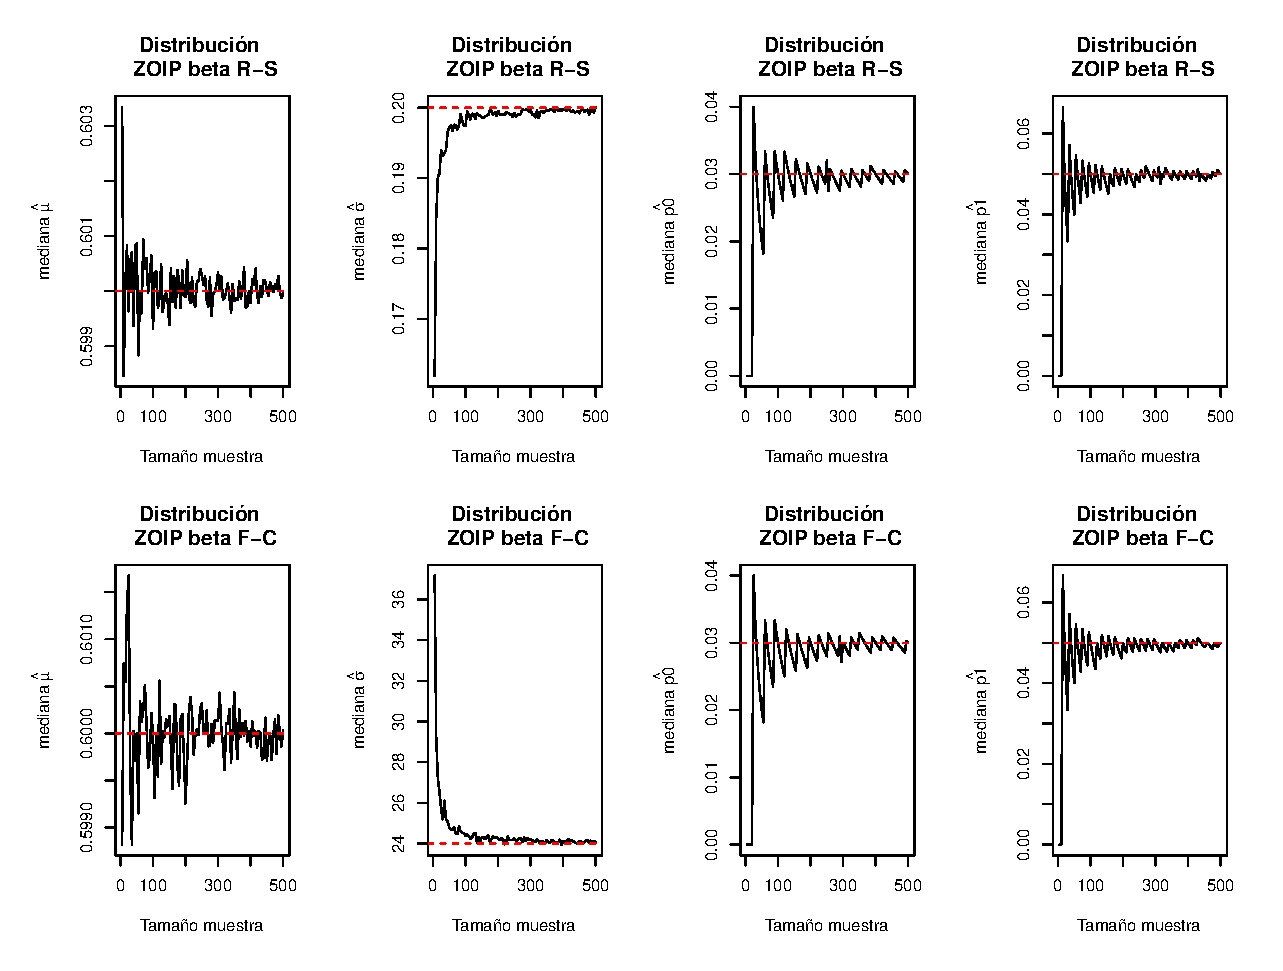
\includegraphics[scale=0.55]{Simulacion_RS_FC.eps}
		\quad
		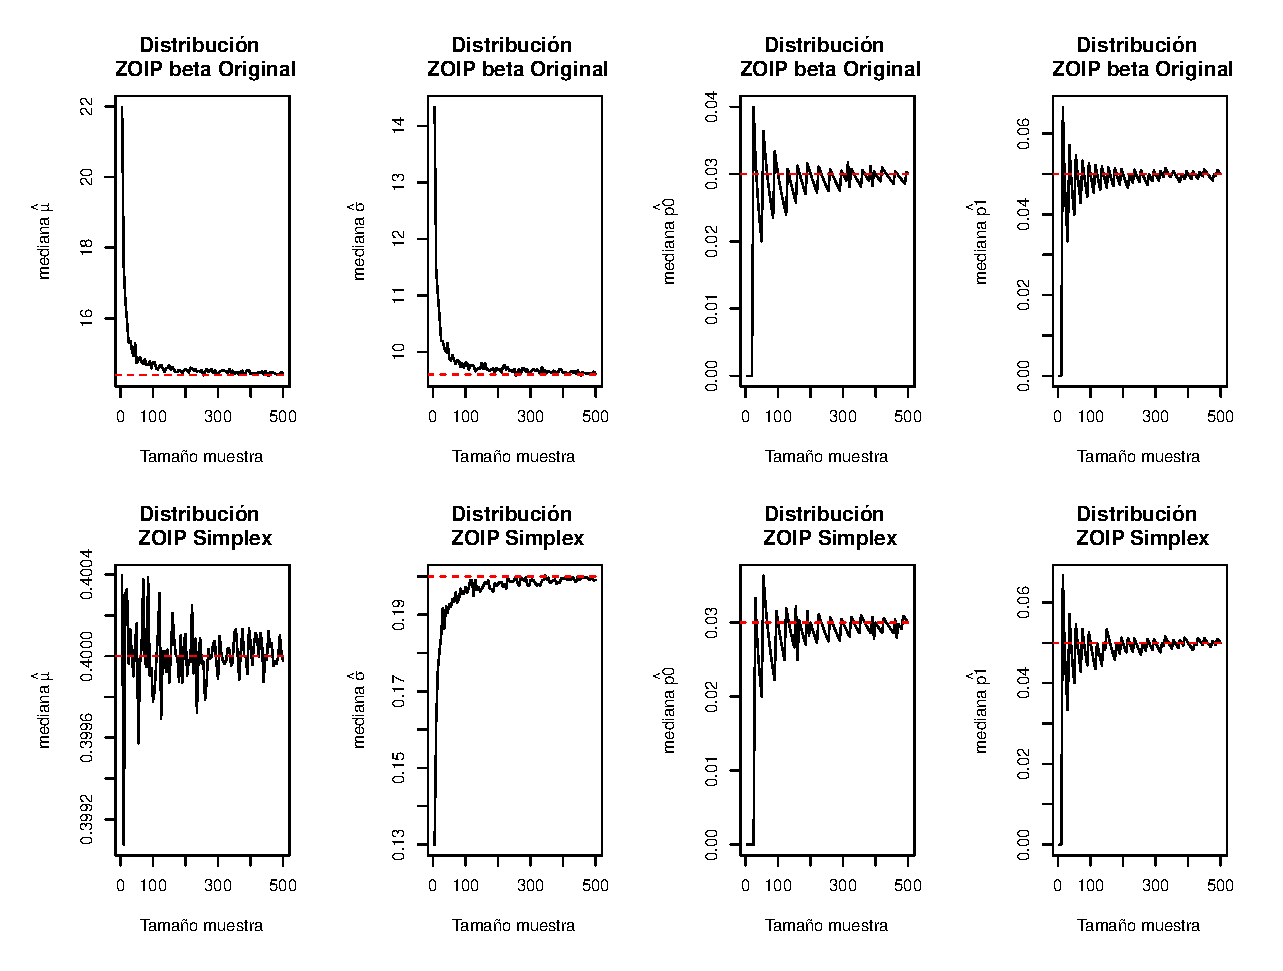
\includegraphics[scale=0.55]{Simulacion_Ori_Sim.eps}	
		\caption{Mediana de los par\'{a}metros estimados en el escenario 1 para distintas parametrizaciones y valores de $n$, las l\'{\i}neas rojas representan el verdadero valor del par\'{a}metro.}
		\label{Simu_1}
	\end{center}
\end{figure}

En la Figura \ref{Simu_1} se presentan las medianas de la estimaci\'{o}n de los par\'{a}metros para cada tama\~{n}o de muestra, de esta figura se observa que independientemente de la distribuci\'{o}n y pa\-ra\-me\-tri\-za\-ci\-\'{o}n escogida en la distribuci\'{o}n ZOIP, todos las estimaciones convergen al valor verdadero del par\'{a}metro a medida que aumenta el tama\~{n}o de muestra n, de la Figura \ref{Simu_1} se nota que las estimaciones de $\sigma$ cuando son par\'{a}metros con significado de dispersi\'{o}n como es en la distribuci\'{o}n beta con parametrizaci\'{o}n \cite{Stasinopoulos2} y en la distribuci\'{o}n simplex, tienden a dar valores subestimados, por otra parte, en las distribuciones que $\sigma$ tiene significado de forma y precisi\'{o}n tienden a dar valores sobrestimados. Se observa que las estimaciones de los par\'{a}metros de inflaci\'{o}n a pesar de que son peque\~{n}as dan resultados muy satisfactorios y casi sin variaci\'{o}n en su forma de estimaci\'{o}n de distribuci\'{o}n a distribuci\'{o}n.\\

Como medida global del proceso de estimaci\'{o}n se eligi\'{o} el MAPE (Error porcentual absoluto medio. $(\sum_{i=1}^{n}{|y_i-\hat{y}_i/y_i}|)/n$) debido a los cambios de escala entre los diferentes par\'{a}metros de las diferentes distribuciones y parametrizaciones. Esta media se realiz\'{o} como un promedio de los MAPES generados por cada uno de los par\'{a}metros de la distribuci\'{o}n ZOIP en cada tama\~{n}o de muestra. En la Figura \ref{Mapes}a se presenta el MAPE para las diferentes distribuciones y parametrizaciones estimadas, se observa como a medida que el tama\~{n}o de muestra aumenta, el MAPE va decreciendo r\'{a}pidamente, aunque des\-pu\'{e}s de un tama\~{n}o de muestra de 200, el MAPE decrece de una manera m\'{a}s lenta, adem\'{a}s los errores de estimaci\'{o}n son muy parecidos entre los cuatro casos de simulaci\'{o}n, la estimaci\'{o}n sobre los par\'{a}metros de la distribuci\'{o}n ZOIP-simplex tiene un error un poco m\'{a}s grande, pero no es significativo sobre los dem\'{a}s casos.\\
 
En el segundo escenario de simulaci\'{o}n se gener\'{o} el mismo ejercicio de simulaci\'{o}n anterior sobre las mismas distribuciones y parametrizaciones, solo que los valores de $p_0$ y $p_1$ cambian por $0.3$ y $0.2$, respectivamente. Dando as\'{\i} que el 50\% de los datos se vean contaminados por ceros y unos, esto para ver si de alguna forma afecta el aumento de la presencia de ceros y unos sobre las estimaciones de los par\'{a}metros de la parte continua de la distribuci\'{o}n ZOIP.

\begin{figure}
	\begin{center}
		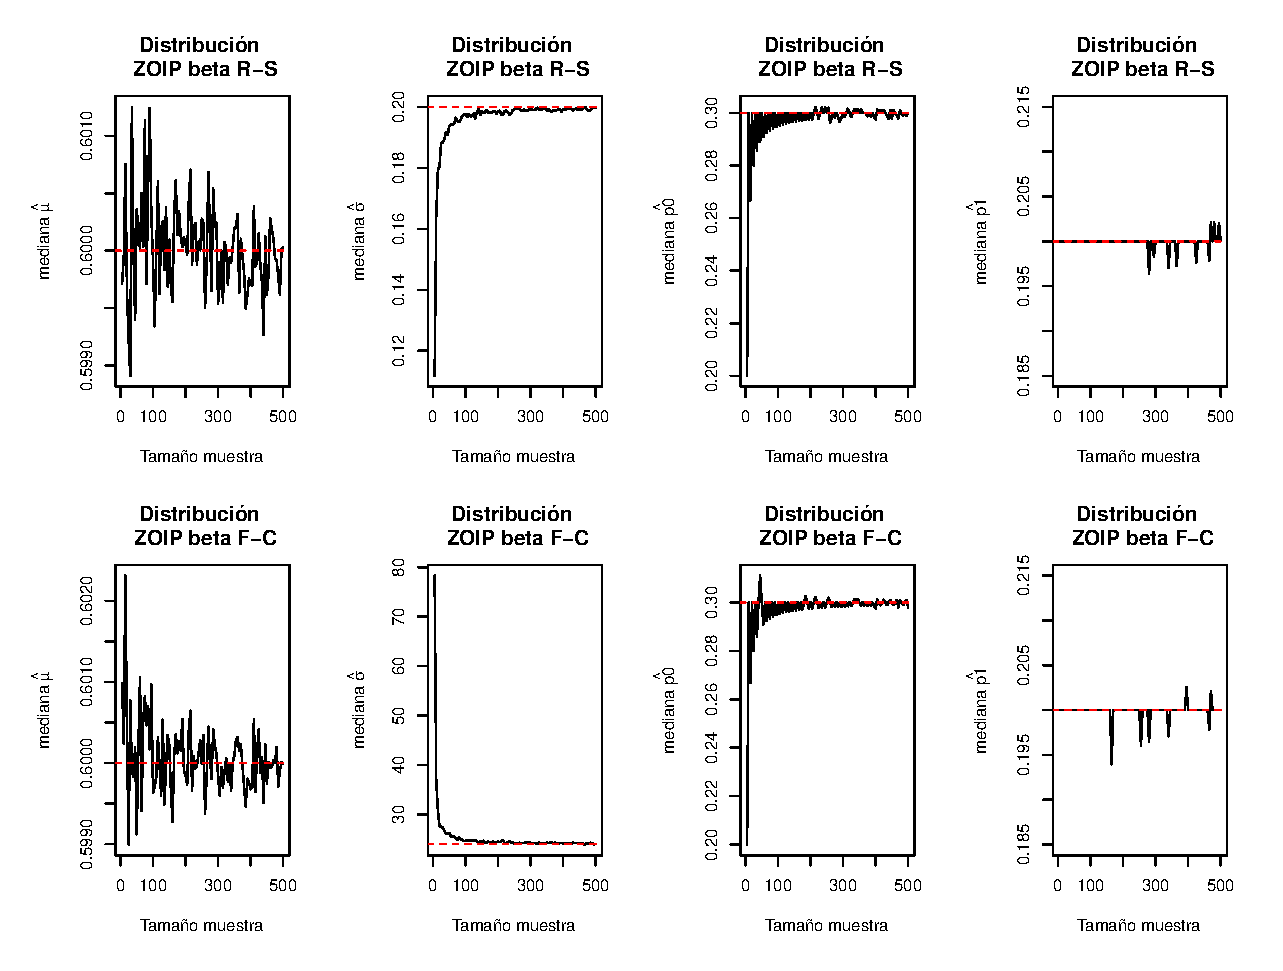
\includegraphics[scale=0.55]{Simulacion_RS_FC_Infla.eps}
		\quad
		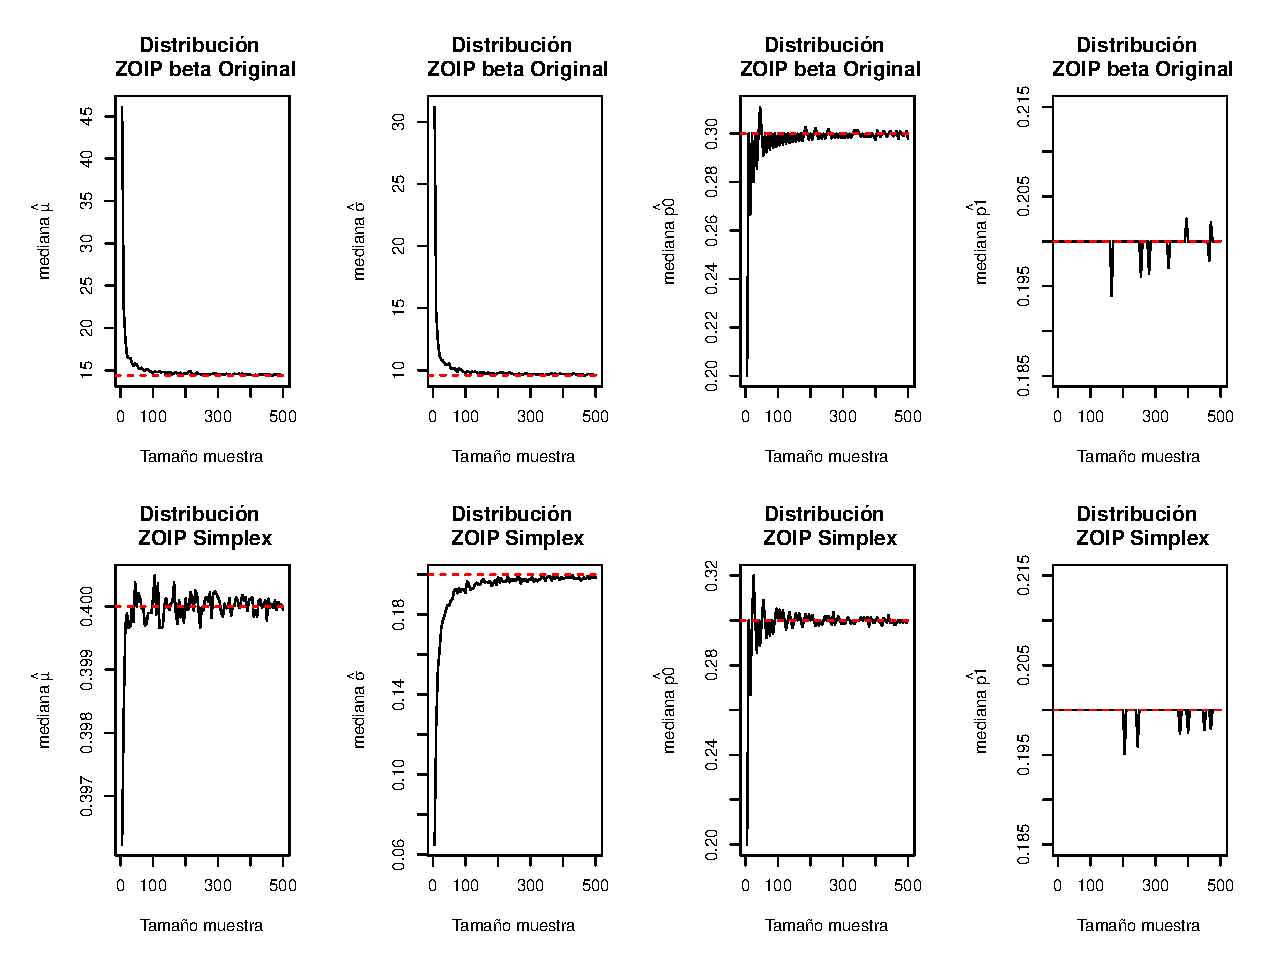
\includegraphics[scale=0.55]{Simulacion_Ori_Sim_Infla.eps}	
		\caption{Simulaci\'{o}n de distribuci\'{o}n ZOIP para distintas par\'{a}metrizaciones con pa\-r\'{a}\-me\-tros de inflaci\'{o}n grandes, distribuciones y valores de $n$.}
		\label{Simu_2}
	\end{center}
\end{figure}

En la Figura \ref{Simu_2} se presentan las estimaciones de los par\'{a}metros de la simulaci\'{o}n con inflaciones al 50\% para diferentes tama\~{n}os de muestras, en general se observa que no se ven cambios muy significativos sobre la Figura \ref{Simu_1} en los par\'{a}metros de $\mu$ y $\sigma$, sin embargo, en la estimaci\'{o}n de $p_0$ se tienden a dar valores subestimados con relaci\'{o}n al estudio de simulaci\'{o}n anterior y con el par\'{a}metro $p_1$ aunque las estimaciones son muy acertadas sobre el valor real desde tama\~{n}os de muestra peque\~{n}os, en algunas ocasiones se producen peque\~{n}as perturbaciones no muy alejados del valor real.


\begin{figure}
	\begin{center}
		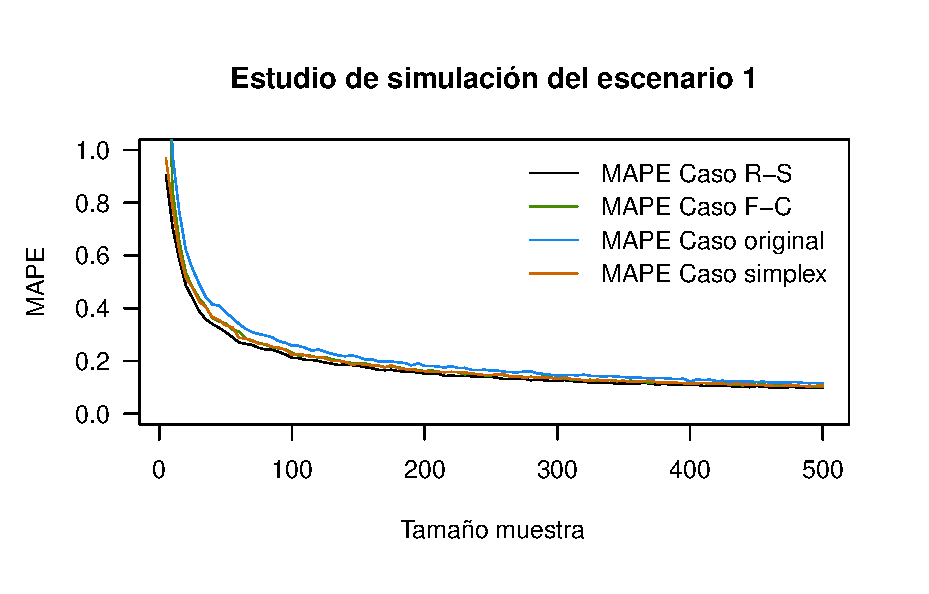
\includegraphics[scale=0.45]{Mape_gnrl.eps}	
		\quad
		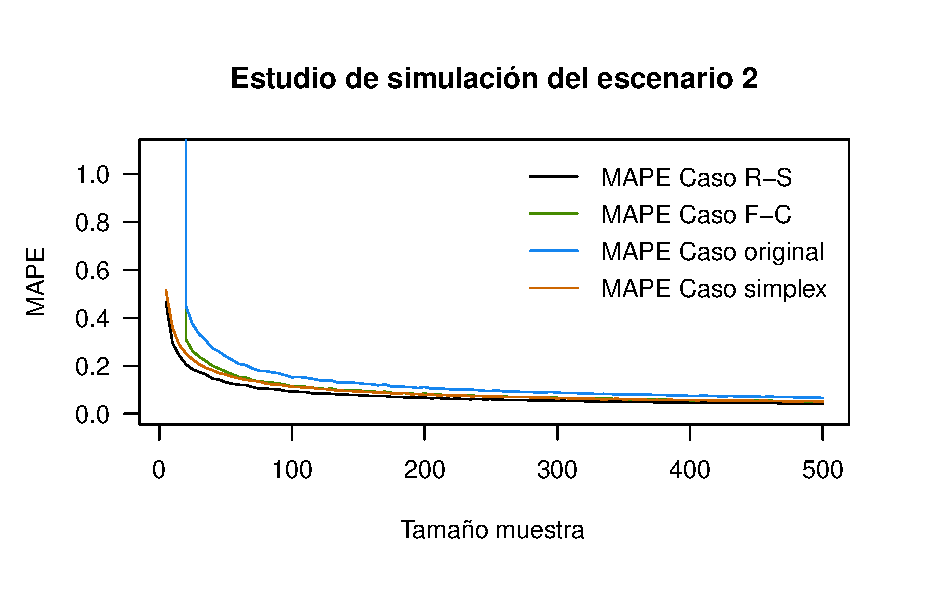
\includegraphics[scale=0.45]{Mape_gnrl_infla.eps}
		\caption{MAPE (Error porcentual absoluto medio) para los dos escenarios de simulaci\'{o}n y para distintas parametrizaciones y valores de $n$.}
		\label{Mapes}
	\end{center}
\end{figure}

\begin{table}[!hbt]
{\scriptsize
\begin{center}
\begin{tabular}{|c|l|cc|}\hline
 Par\'{a}metro & Caso & MAPE escenario 1 \% &  MAPE escenario 2 \% \\ \hline

\multirow{4}{*}{$\mu$}&Caso R-S &0.61 & 0.86	\\
& Caso F-C & 0.50	& 0.85	\\
& Caso original &0.53 & 0.70	 \\
& Caso simplex 	&0.47 & 0.63	\\ \hline

\multirow{4}{*}{$\sigma$} &Caso R-S &2.53 & 3.40\\
& Caso F-C 	&5.10 & 6.90\\
& Caso original &5.30 & 6.98\\
& Caso simplex 	&5.30  &7.37 \\\hline

\multirow{4}{*}{$p_0$} &Caso R-S &20.5  & 5.36	\\
& Caso F-C &19.7  & 5.42	\\
& Caso original &19.8 & 5.43	\\
& Caso simplex 	&20.8 & 5.51\\ \hline

\multirow{4}{*}{$p_1$} &Caso R-S 	&15.2 & 7.28\\
& Caso F-C &16.0 & 7.00  \\
& Caso original &15.7	 & 7.00	\\
& Caso simplex &16.2 & 7.12	 \\ \hline
& Promedio & 10.57 & 5.26 \\ \hline
\end{tabular}
\caption{MAPE de las estimaciones para cada par\'{a}metro en diferentes parametrizaciones en los dos estudios de simulaci\'{o}n.}
\label{T_MAPES}
\end{center}
}
\end{table}

En la Figura \ref{Mapes}b se presenta el MAPE para el estudio de simulaci\'{o}n del escenario 2, se puede ver como se obtienen MAPES muy parecidos a los del estudio de simulaci\'{o}n del escenario 1, pero cabe resaltar como se comete menos error sobre la estimaci\'{o}n de los par\'{a}metros de la distribuci\'{o}n beta con parametrizaci\'{o}n \cite{Stasinopoulos2}. En la tabla \ref{T_MAPES} se presenta el MAPE para cada par\'{a}metro de cada parametrizaci\'{o}n para ambos estudios de simulaci\'{o}n, es claro ver como en general el estudio de simulaci\'{o}n del escenario 2 produce un MAPE menor que el del escenario 1, esto es causado por que en el escenario 1 de simulaci\'{o}n los errores de pron\'{o}stico son m\'{a}s grandes en los par\'{a}metros de inflaci\'{o}n que en el escenario 2. Por todo lo visto anteriormente se puede concluir que el crecimiento de los par\'{a}metros de inflaci\'{o}n no afecta de manera significativa la estimaci\'{o}n de los par\'{a}metros de la parte continua de la distribuci\'{o}n ZOIP, pero si en una mejor estimaci\'{o}n de los par\'{a}metros de inflaci\'{o}n.


\subsection{Datos reales}
En esta secci\'{o}n se presenta el ajuste de una distribuci\'{o}n ZOIP a datos reales sobre la utilizaci\'{o}n de una tarjeta de cr\'{e}dito en un banco, para una entidad financiera grande como un banco es de vital importancia conocer el comportamiento del porcentaje de utilizaci\'{o}n de sus tarjetas de cr\'{e}dito (tdc), se define a $y$ como el porcentaje de uso de una tdc, en la Figura \ref{hist_tdc} se presenta el histograma del porcentaje de utilizaci\'{o}n de las tdc y es claro notar que $y$ se encuentra entre cero y uno, pero adicional es muy com\'{u}n ver que las tdc no sean utilizadas ($y=0$) y tambi\'{e}n que las tdc sean utilizadas en la totalidad de su cupo asignado ($y=1$), por lo que se trata a $y$ como una variable aleatoria perteneciente a datos proporcionales inflados con ceros y unos. Se tiene un total de $9206$ tdc, que representan el porcentaje de utilizaci\'{o}n de las tdc para un trimestre del a\~{n}o 2014 del banco. Se quiere estudiar el ajuste de una distribuci\'{o}n ZOIP, para ello se utiliza el paquete en \proglang{R} llamado \pkg{ZOIP} mediante su funci\'{o}n \code{RM.ZOIP}.\\

\begin{figure}
	\begin{center}
		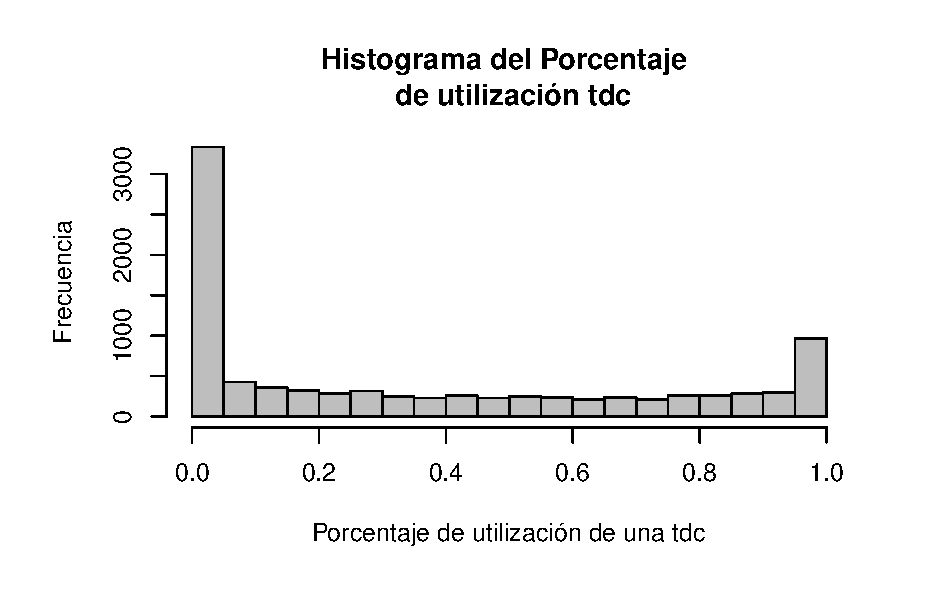
\includegraphics[scale=0.6]{Hist_tdc.eps}
		\caption{Histograma del porcentaje de utilizaci\'{o}n de las tdc en un banco.}
		\label{hist_tdc}
	\end{center}
\end{figure}

\begin{table}[!hbt]
{\scriptsize
\begin{center}
\begin{tabular}{|c|c|ccc|c|}\hline
Familia & Par\'{a}metro & Estimaci\'{o}n & Error est\'{a}ndar & Valor P & Log-Verosimilitud\\ \hline

\multirow{4}{*}{R-S} &$\mu$ &0.4040	&0.0037	&$<2.2e^{-16}$ &\multirow{4}{*}{5854.067}\\
& $\sigma$ & 0.6601	&0.0027	&$<2.2e^{-16}$& \\
& $p_0$ & 0.2219	&0.0043	&$<2.2e^{-16}$ &\\
& $p_1$ & 0.0695	&0.0027	&$<2.2e^{-16}$ &\\ \hline

\multirow{4}{*}{F-C} &$\mu$ & 0.4040	&0.0037	&$<2.2e^{-16}$ &\multirow{4}{*}{5854.067}\\
& $\sigma$ & 0.4040	&0.0037	&$<2.2e^{-16}$ &\\
& $p_0$ & 0.2219	&0.0043	&$<2.2e^{-16}$ &\\
& $p_1$ & 0.0695	&0.0027	&$<2.2e^{-16}$ &\\ \hline

\multirow{4}{*}{original} &$\mu$ & 0.5233	&0.0080	&$<2.2e^{-16}$&\multirow{4}{*}{5854.067} \\
& $\sigma$ & 0.7719	&0.0130	&$<2.2e^{-16}$& \\
& $p_0$ & 0.2219	&0.0043	&$<2.2e^{-16}$& \\
& $p_1$ & 0.0695	&0.0027	&$<2.2e^{-16}$& \\ \hline

\multirow{4}{*}{simplex} &$\mu$ & 0.5741	&0.0010	&$<2.2e^{-16}$ &\multirow{4}{*}{54425.63}\\
& $\sigma$ & 4885.44	&18.2430	&$<2.2e^{-16}$ &\\
& $p_0$ & 0.1497	&0.0032	&$<2.2e^{-16}$ &\\
& $p_1$ & 0.0090	&0.0004	&$<2.2e^{-16}$ &\\ \hline

\end{tabular}
\caption{Ajuste de diferentes distribuciones ZOIP en el porcentaje de utilizaci\'{o}n de una tdc.}
\label{T_Apli_SC}
\end{center}
}
\end{table}


En la Tabla \ref{T_Apli_SC} se muestran resultados de los cuatro par\'{a}metros estimados v\'{\i}a m\'{a}xima verosimilitud para la distribuci\'{o}n ZOIP, en ellas vemos c\'{o}mo cambian los valores de los par\'{a}metros seg\'{u}n la parametrizaci\'{o}n escogida, los valores de log-verosimilitud no indican que el mejor modelo ajustado es un ZOIP-beta, ya que es bastante menor el valor de log-verosimilitud de una distribuci\'{o}n ZOIP-simplex, adem\'{a}s que en las estimaciones de los par\'{a}metros de la distribuci\'{o}n ZOIP-simplex no se tuvo una convergencia, por lo tanto los valores son muy distintos para el par\'{a}metro de dispersi\'{o}n a los vistos en la distribuci\'{o}n ZOIP-beta, inclusive muy elevados. Adem\'{a}s, el valor de $\mu$ es mayor que las de la parametrizaci\'{o}n en \cite{Stasinopoulos2} y \cite{Ferrari2}, un 17\% m\'{a}s.\\

\begin{figure}
	\begin{center}
		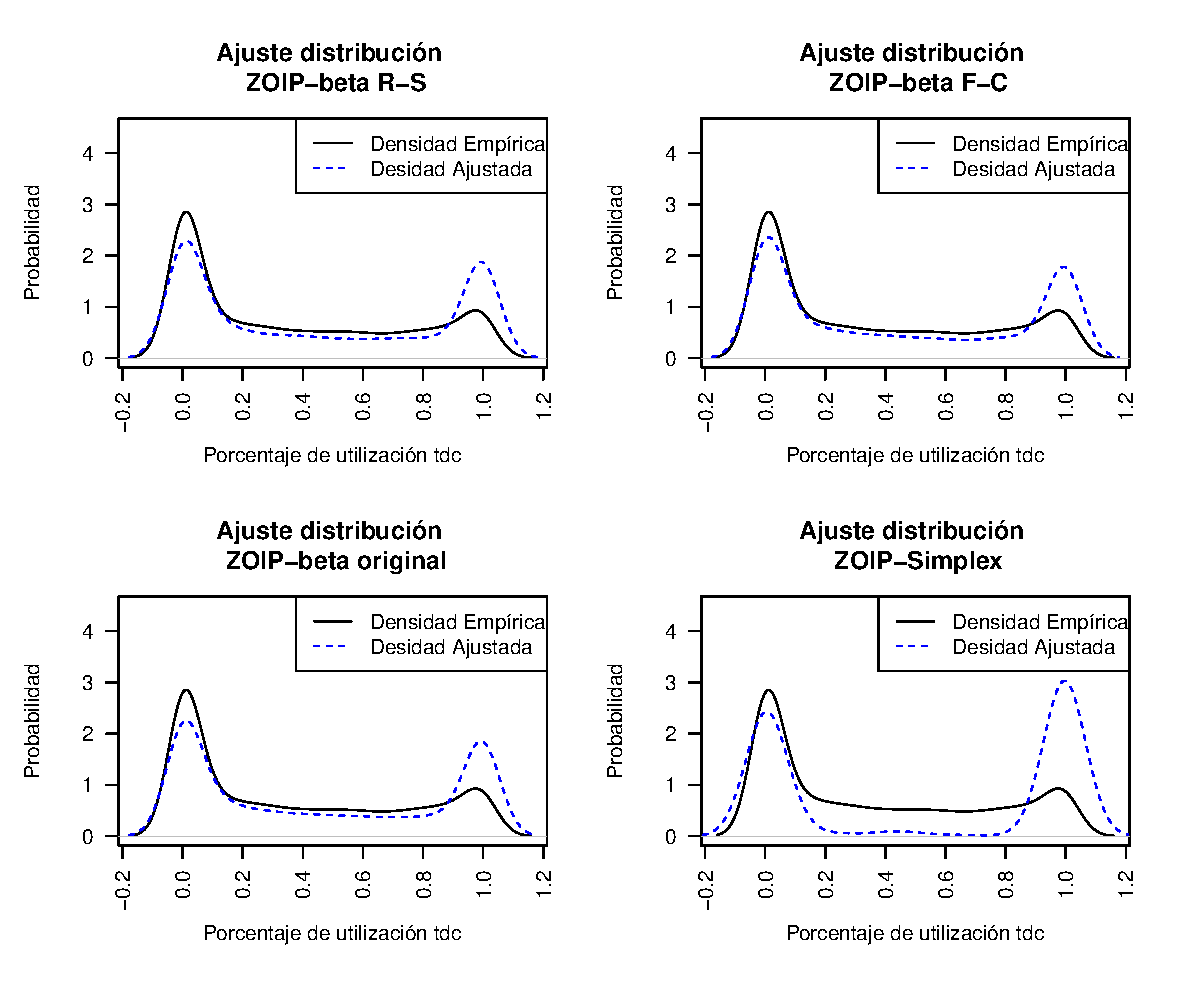
\includegraphics[scale=0.55]{Aplicacion_SC.eps}
		\caption{Ajuste de diferentes distribuciones y parametrizaciones ZOIP al porcentaje de utilizaci\'{o}n de una tdc.}
		\label{Apli_Aju_ZOIP}
	\end{center}
\end{figure}


En la Figura \ref{Apli_Aju_ZOIP} se presenta gr\'{a}ficamente el ajuste de la distribuci\'{o}n ZOIP para diferentes parametrizaciones al porcentaje de utilizaci\'{o}n de las tdc, la l\'{\i}nea azul que representa la distribuci\'{o}n ZOIP ajustada, es de notar que dicha l\'{\i}nea azul es exactamente igual en las tres ocasiones que se ajusta la distribuci\'{o}n ZOIP-beta y se ve como sigue el comportamiento original del porcentaje de utilizaci\'{o}n de las tdc. Es bueno resaltar tambi\'{e}n como en la Figura 1d de la Figura \ref{Apli_Aju_ZOIP} no se nota un buen ajuste para los valores entre cero y uno. Por todo anterior es recomendable decir que el porcentaje de utilizaci\'{o}n de las tdc de este banco se comportan como una distribuci\'{o}n ZOIP-beta con los par\'{a}metros descritos en la tabla \ref{T_Apli_SC}, seg\'{u}n la parametrizaci\'{o}n deseada y no como una distribuci\'{o}n ZOIP-simplex.

%%%%%%%%%%%%%%%%%%%%%%%%%%%%%%%%%%%%%%%%%%%%%%%%%%%%%%%%%%%%%%%%%%%%%%%%%%%%%%%%%%%%%%%%%%%%%%%%%%%%%%%%%%%%%%%%%%%%%%%%%%%%%%%%%%%%%%%%%%%%%%%%%%%%%%%%%%%%%%%%%%

\section{Conclusiones}

La distribuci\'{o}n ZOIP y el paquete \pkg{ZOIP} de \proglang{R} permiten ajustar distribuciones para datos provenientes de porcentajes, tasas o proporciones que se encuentren inflados con ceros y/o unos, dicha distribuci\'{o}n est\'{a} compuesta por cuatro par\'{a}metros, que son estimados v\'{\i}a m\'{a}xima verosimilitud y en el cual de acuerdo a los estudios de simulaci\'{o}n realizados estos convergen a los valores reales con un tama\~{n}o de muestra relativamente peque\~{n}o, adem\'{a}s se observa como la estimaci\'{o}n de los par\'{a}metros de la parte continua no se ven afectados por el aumento de la presencia de ceros y unos en los datos, pero si la estimaci\'{o}n de los par\'{a}metros de la parte discreta. Por otra parte, se observa como el Ajuste de la distribuci\'{o}n ZOIP-beta explica el comportamiento de la distribuci\'{o}n del porcentaje de utilizaci\'{o}n de una tarjeta de cr\'{e}dito en un banco.\\

La distribuci\'{o}n ZOIP y el paquete \pkg{ZOIP} de \proglang{R} permiten de una manera muy vers\'{a}til utilizar y ajustar diferentes parametrizaciones y distribuciones para datos proporcionales. Adem\'{a}s permite Utilizar y ajustar distribuciones para datos proporcionales que se encuentran inflados solo con ceros o solo con unos, de una manera pr\'{a}ctica.
